% 图 7.6 (a) k 空间点阵（同 7.1a）(b) 朗道能级：同心圆 k_l，加黑圆环面积 πk_{l+1}^2−πk_l^2
\documentclass[tikz,border=5pt]{standalone}
\usetikzlibrary{arrows.meta}
\usepackage{amsmath}
\usepackage{bm}
\usepackage{fontspec}
\setmainfont{Times New Roman}
\begin{document}
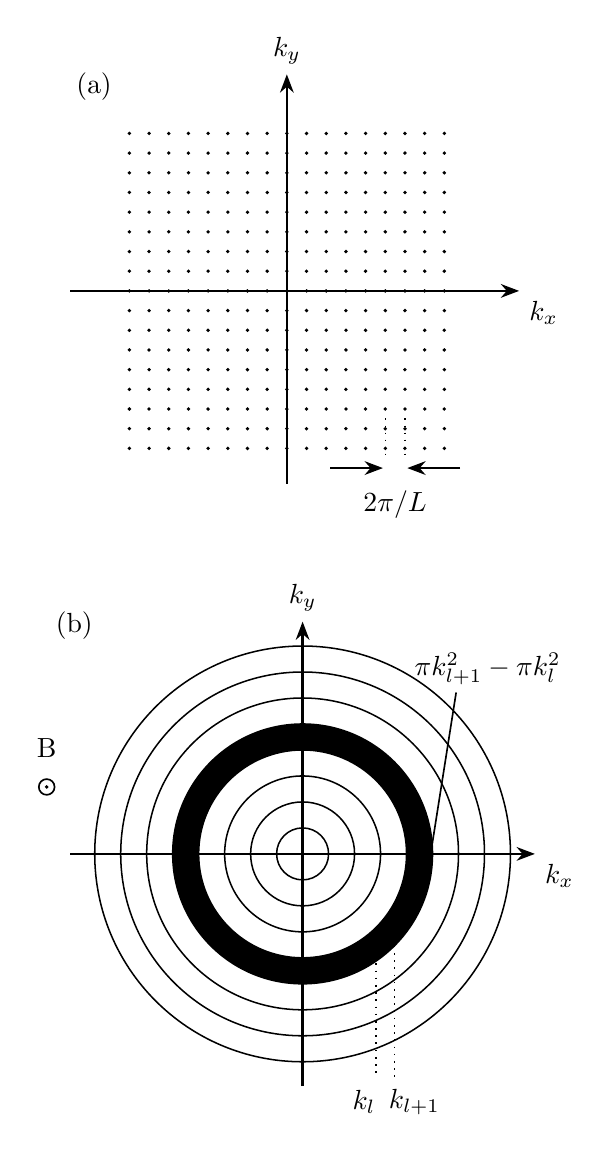
\begin{tikzpicture}[line width=0.8pt,>=Stealth]
% ---------- (a) 点阵 ----------
\begin{scope}
\node at (-2.45,2.6) {(a)};
\foreach \i in {-8,...,8}
  \foreach \j in {-8,...,8}
    \fill (\i*0.25,\j*0.25) circle (0.024);
\draw[->] (0,-2.45) -- (0,2.75) node[above] {$k_y$};
\draw[->] (-2.75,0) -- (2.95,0) node[below right] {$k_x$};
\draw[dotted,line width=0.55pt] (1.25,-1.62) -- (1.25,-2.1);
\draw[dotted,line width=0.55pt] (1.5,-1.62) -- (1.5,-2.1);
\draw[->] (0.55,-2.25) -- (1.22,-2.25);
\draw[->] (2.2,-2.25) -- (1.53,-2.25);
\node at (1.375,-2.72) {$2\pi/L$};
\end{scope}
% ---------- (b) 朗道同心圆 ----------
\begin{scope}[shift={(0.2,-7.15)}]
\node at (-2.9,2.9) {(b)};
% 8 个同心细圆，间距 0.33
\foreach \r in {1,...,8}
  \draw[line width=0.55pt] (0,0) circle (\r*0.33);
% 加黑圆环：第 4-5 圆之间
\fill[even odd rule] (0,0) circle (1.65) (0,0) circle (1.32);
% 坐标轴
\draw[->] (-2.95,0) -- (2.95,0) node[below right] {$k_x$};
\draw[->] (0,-2.95) -- (0,2.95) node[above] {$k_y$};
% 环面积标签（斜引线指向黑环右下缘）
\node at (2.35,2.35) {$\pi k_{l+1}^{2}-\pi k_l^{2}$};
\draw[line width=0.6pt] (1.95,2.05) -- (1.56,-0.42);
% B 与 ⊙（垂直纸面向外）
\node at (-3.25,1.35) {$\mathrm{B}$};
\draw[line width=0.6pt] (-3.25,0.85) circle (0.1);
\fill (-3.25,0.85) circle (0.025);
% 黑环下缘两条竖直点线 → k_l, k_{l+1}
\draw[dotted,line width=0.6pt] (0.933,-0.933) -- (0.933,-2.85);
\draw[dotted,line width=0.6pt] (1.167,-1.167) -- (1.167,-2.85);
\node at (0.78,-3.15) {$k_l$};
\node at (1.42,-3.15) {$k_{l+1}$};
\end{scope}
\end{tikzpicture}
\end{document}
